\documentclass[14pt]{extarticle}

\usepackage[english]{babel}
\usepackage[utf8]{inputenc}
\usepackage{hyperref}
\usepackage{graphicx,eso-pic}
\usepackage{newtxtext}
\usepackage{setspace}
\usepackage{multirow}
\usepackage{array}
\usepackage{lipsum}
\usepackage{titlesec}
\usepackage{multicol}
\usepackage{pdfpages}
\usepackage{indentfirst}
\usepackage[bottom=1.5cm,top=2.5cm,left=2cm,right=2cm]{geometry}

\hypersetup{
    colorlinks=true,
    linkcolor=black,
    filecolor=magenta,      
    urlcolor=blue,
    pdftitle={Synopsis},
    pdfpagemode=FullScreen,
    }

\urlstyle{same}

\makeatletter

\setlength{\parskip}{1em}

\newcommand\frontmatter{
    \cleardoublepage
    \pagenumbering{roman}
}

\newcommand\mainmatter{
    \cleardoublepage
    \pagenumbering{arabic}
}

\newcommand\backmatter{
    \if @openright
        \cleardoublepage
    \else
        \clearpage
    \fi
}

\makeatother

\titleformat{\section}[block]{\Large\bfseries\filcenter}{}{1em}{}


\title{Federated Learning With IoT Devices}
\author{}
\date{}

\begin{document}

\frontmatter

\newgeometry{bottom=2cm,top=2cm,left=1.5cm,right=1.5cm}
\addcontentsline{toc}{section}{Title}
\vspace{-7em}
\maketitle

\vspace{-7em}

\begin{center}
    \singlespacing
\textbf {A Project Work Synopsis} \\ 

\vspace{1cm}
\onehalfspacing
\emph {Submitted in partial fulfilment for the award of the degree of} \\ 

\vspace{1.5cm}
\singlespacing

\textbf{
BACHELOR OF ENGINEERING \\
IN \\
COMPUTER SCIENCE and ENGINEERING - INTERNET of THINGS\\
}

\vspace{2.5em}
\onehalfspacing
\textbf{
Submitted by : \\
\begin{tabular}{ccccc}
    Rishabh Anand & Udita Mitra & Vandana Chauhan & Khushwant Rathore & Abhishek Gupta \\
    19BCS4525 & 19BCS4662 & 19BCS4532 & 19BCS4644 &  19BCS4579 \\
\end{tabular}
}

\textbf{
Under the Supervision of : \\
Piyush Samanth
}

\vspace{1em}

\includegraphics[scale=0.25]{private/seal.png}

\singlespacing

CHANDIGARH UNIVERSITY, GHARUAN, MOHALI - 140413\\
Punjab

\onehalfspacing
August, 2021

\end{center}
\restoregeometry

\newpage

\newpage
\addcontentsline{toc}{section}{Timeline}

\section*{Timeline}
\begin{center}
    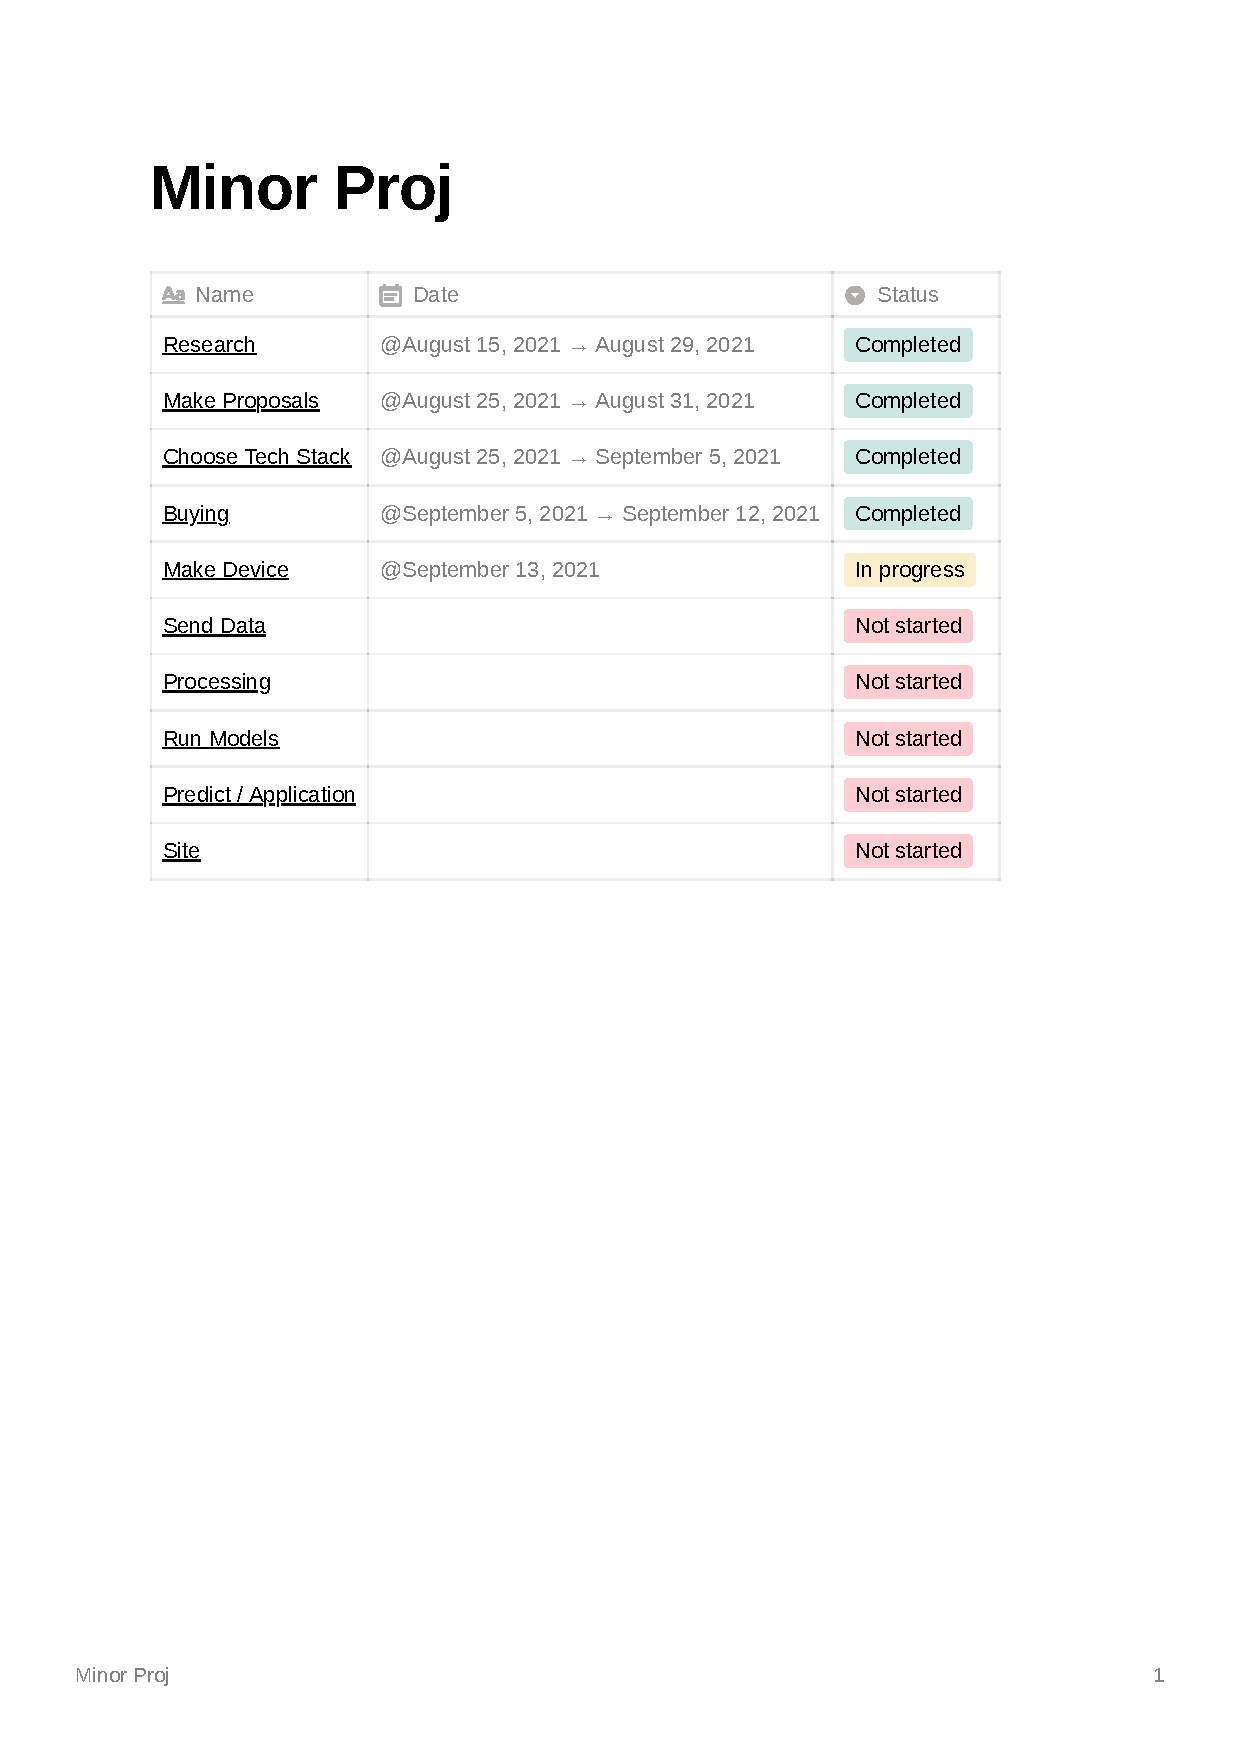
\includegraphics[width=.75\textwidth]{private/gantt.png}
    \includegraphics[width=.75\textwidth]{private/gantt2.png}
\end{center}


\newpage
\addcontentsline{toc}{section}{List of figures}
\listoffigures

\newpage
\addcontentsline{toc}{section}{List of tables}
\listoftables

\setlength{\parskip}{0em}
\newpage
\addcontentsline{toc}{section}{CONTENTS}
\begin{center}
    \tableofcontents
\end{center}

\mainmatter

\setlength{\parskip}{1em}

\newpage
\section{INTRODUCTION}

\par The rapid development of Internet of Things (IoT) systems has led to the problem ofmanaging and analyzing the large volumes of data that they generate. Traditional approaches that involve collection of data from IoT devices into one centralized repository for further analysis are notalways applicable due to the large amount of collected data, the use of communication channels with limited bandwidth, security and privacy requirements, etc.

\par Federated learning (FL) is an emerging approach that allows one to analyze data directly on data sources and to federate the results of eachanalysis to yield a result as traditional centralized data processing. FL is being actively developed,and currently, there are several open-source frameworks that implement it.

\subsection{Project Definition}

\par This project presents a demonstration of Federated Learning after an extensive and comparative review and analysis of the existing open-source FL frameworks, including their applicability in IoT systems.

We evaluated the following features of the frameworks: 
\begin{itemize}
    \item Ease of use and deployment
    \item Development
    \item Analysis capabilities
    \item Accuracy
    \item Performance
\end{itemize}

The data set was prepared in-house using MAX30100/02/05 sensors. To model low-power IoT devices, computing nodes with small resources were defined inthe test bed. The research results revealed FL frameworks that could be applied in the IoT systems now, but with certain restrictions on their use.

\newpage
\subsection{Project Overview}

\par In the world of all-things-smart, everything is being run on data. Anything that we 
see is data and everything that we use either generates or uses data. Data can comprise of
anything, ranging from the weather details of your city to your personal health details.
The data generated, may contain sensitive information about an individual or even an
organization. If the owner has to share there data with various other groups of people for
various reasons like analysis. A link of the data is then made available to the person of
choice in encrpyted form.

\par Looking at this from a developers perspective, we may need data from different sources
to fully complete our analysis and give meaningful results. But since we don’t have the
data at one place, it becomes a really difficult task to use any particular mode of training.
Well any mode other than FEDERATED LEARNING. Federated Learning is a very good
way to use sensitive data from different parties who are not willing to disclose their exact
data.

\par In our case, we are using a custom built oximeter to generate data and then analysis the
Heart Rate and SPO2 of different individuals and then predict things like who has a higher
chance of getting a heart attack and who is running low on SPO2. Now, people may not
want to share their heart rate information with general public, so instead they hash their
reading before passing the information. We then aggregate that data onto our process and
then, predict the desired information and keep the private information private.

\newpage
\subsection{Hardware Specification}
\subsubsection{ESP32}
\singlespacing

\par ESP32 is a series of low-cost, low-power system on a chip microcontrollers with integrated Wi-Fi and dual-mode Bluetooth. The ESP32 series employs either a Tensilica Xtensa LX6 microprocessor in both dual-core and single-core variations, Xtensa LX7 dual-core microprocessor or a single-core RISC-V microprocessor and includes built-in antenna switches, RF balun, power amplifier, low-noise receive amplifier, filters, and power-management modules. ESP32 is created and developed by Espressif Systems, a Shanghai-based Chinese company, and is manufactured by TSMC using their 40 nm process.

The esp32 chip used in our expriments and project had :
\begin{itemize}
    \item 2 CPU core(s)
    \item WiFi/BT/BLE
    \item Silicon revision 1
    \item 2MB external flash
    \item Minimum free heap size: 294448 bytes
\end{itemize}

The ESP32 Board can be used in conjuction of Arduino or as a stand- alone board. It can be programmed by using Arduino-IDE or by using Espressif-IDF given by it's makers.

\begin{figure}[!h]
    \centering
    \includegraphics[width=0.45\textwidth]{private/esp.jpg}
    \caption{ESP32}
    \label{fig:esp}
\end{figure}

\subsubsection{MAX30100/02/05}

\par The MAX30102 is an integrated pulse oximetry and heart-rate monitor biosensor module based on PPG ((PhotoPlethysmoGraphy). It is so small that you can just wear it on your finger or wrist for data collecting. Internally integrated 18bit ADC, the sensor supports I2C data output, which could be compatible for most controllers.

\begin{multicols}{2}
    Features :
    \begin{itemize}
        \item Extremely low standby current
        \item High sampling rate
        \item High SNR
    \end{itemize}
    
    
    Application :
    \begin{itemize}
        \item Heart-rate Measurement
        \item SPO2 Detection
    \end{itemize}
    
    Specification : 
    \begin{itemize}
        \item Power Supply: 3.3V~5V
        \item Working Current: <5mA
        \item RED/IR LED Driving Current: 0-50mA
        \item Communication: I2C
        \item I2C Address: 0x57
        \item Operating Temperature: -40℃~85℃
        \item Dimension: 18×14mm/0.71×0.55”
    \end{itemize}    
\end{multicols}

\vspace{2em}
\begin{figure}[!h]
    \centering
    \includegraphics[width=0.45\textwidth]{private/max.jpg}
    \caption{MAX30100/02/05}
    \label{fig:max}
\end{figure}

\newpage
\subsection{Software Specification}

Tools needed to work with ESP Boards :
\begin{itemize}
    \item Toolchain to compile code for ESP32 (gcc git make flex bison gperf python-pip)
    \item Build tools to build full application (cmake ninja ccache dfu-util libusb)
    \item ESP-IDF
\end{itemize}

\subsubsection{Espressif IDF}

\par ESP-IDF contains the API, software libraries and source code, for ESP32 and scripts to operate the Toolchain. 

\par This can be obtained from espressif's repositories on git. We also need some tools that the idf needs to work. There is an installation script that does all that for us. We then need to set all the installed tools in PATH env variable.

\par With proper permission to access the PORTS, we can also run the build, flash, monitor and see the results, all straight from the terminal.



\newpage
\section{LITERATURE SURVEY}
\subsection{Existing System}
\begin{table}[h!]
    \centering
    \begin{tabular}[]{|m{7em}|m{10em}|m{7em}|m{7em}|}
        \hline
        Title & Comparision & Source & Findings\\
        \hline
        &&&\\
        \multirow{2}{7em}{Distributed Learning} & Different Architechture & Online Papers & Privacy can be increased\\
        & More Secure & Custom Tests& Data Security can be better\\
        &&& \\
        \hline
    \end{tabular}
    \caption{Literature Review summary}
    \label{Table : 1}
\end{table}
\newpage
\subsection{Proposed System}

\par FL as a distributed machine learning paradigm that supports data analysis, such neural network (NN) training, directly on the data storage,only the results of such processing. There are three major components in an FL system:

\begin{enumerate}
    \item Server (e.g., manager).
    \item Communication–computation framework.
    \item Clients (e.g., parties, data sources).
\end{enumerate}

\par FL can treat IID data as non - IID data because training can be performed on sources connected with each other, i.e., sources that store different types of data about the same artifacts or events, or independent data sources. FL uses nodes as data sources and performs calculations as close to the data as possible.
\par The FLDP framework is a very simple open-source framework for FL, which is distributed under the Apache 2.0 license. The framework is developed by Sherpa. This framework implements several aggregation algorithms for different models:
\begin{itemize}
    \item A FedAvg aggregator for NN and LR.
    \item A weighted FedAverage aggregator and IOWA FedAverage aggregator for LR.
    \item A cluster FedAverage aggregator for centroid cluster models.
\end{itemize}

\par The framework implements these privacy mechanisms to protect personal data:
\begin{itemize}
    \item A simple mechanism adding random noise to binary data.
    \item An adaptive differential privacy mechanism based on Privacy Filters.
\end{itemize}

\newpage
\subsubsection{Comparision of Various Framworks}

\begin{figure}[!h]
    \centering
    \includegraphics[width=0.8\textwidth]{private/Diff.png}
    \caption{Comparision of Frameworks}
    \label{fig:comp}
\end{figure}

\begin{figure}[!h]
    \centering
    \includegraphics[width=0.6\textwidth]{private/Chart1.png}
    \caption{Accuracy}
    \label{fig:acc}
\end{figure}

\begin{figure}[!h]
    \centering
    \includegraphics[width=0.6\textwidth]{private/Chart2.png}
    \caption{Training Time}
    \label{fig:time}
\end{figure}


\newpage
\section{PROBLEM FORMULATION}

\par The main objective of this paper  is to design not only a heart rate monitoring system but also to made a Federated System. Federated learning (FL) is a feasible solution to solve the problems of data islands, break data barriers, and protect data security and privacy, especially in the context of the Internet of Things , and big data.

\par Distributed IOT and big data users need to collaboratively train a classification or regression model to implement perfect data prediction results without compromising privacy. Unlike privacy-preserving outsourced training, rather than submitting data to the centralized cloud server, users train data locally in FL. The federated center is only responsible for aggregating the gradient information (or model parameters) uploaded by users and distributing the global training model.

\newpage
\section{RESEARCH OBJECTIVES}

\par Firstly, we have to understand how federated learning (FD) is different from distributed learning.

\begin {itemize}
    \item \par The goal of distributed learning is to scale the parallel processing of a large amount of data, while the purpose of FL is to process data, i.e., train a model, directly on the data sources.
    \item \par Distributed learning works with identically and independently distributed (IID) data, which are collected in a single repository, from which they are extracted for further training. FL can treat IID data as non-IID data because training can be performed on sources connected with each other, i.e., sources that store different types of data about the same artifacts or events, or independent data sources.
    \item \par Another difference is the usage of network nodes. Distributed learning uses network nodes as computing resources for scaling, while FL uses nodes as data sources and performs calculations as close to the data as possible.
\end{itemize}

\begin{figure}[!h]
    \centering
    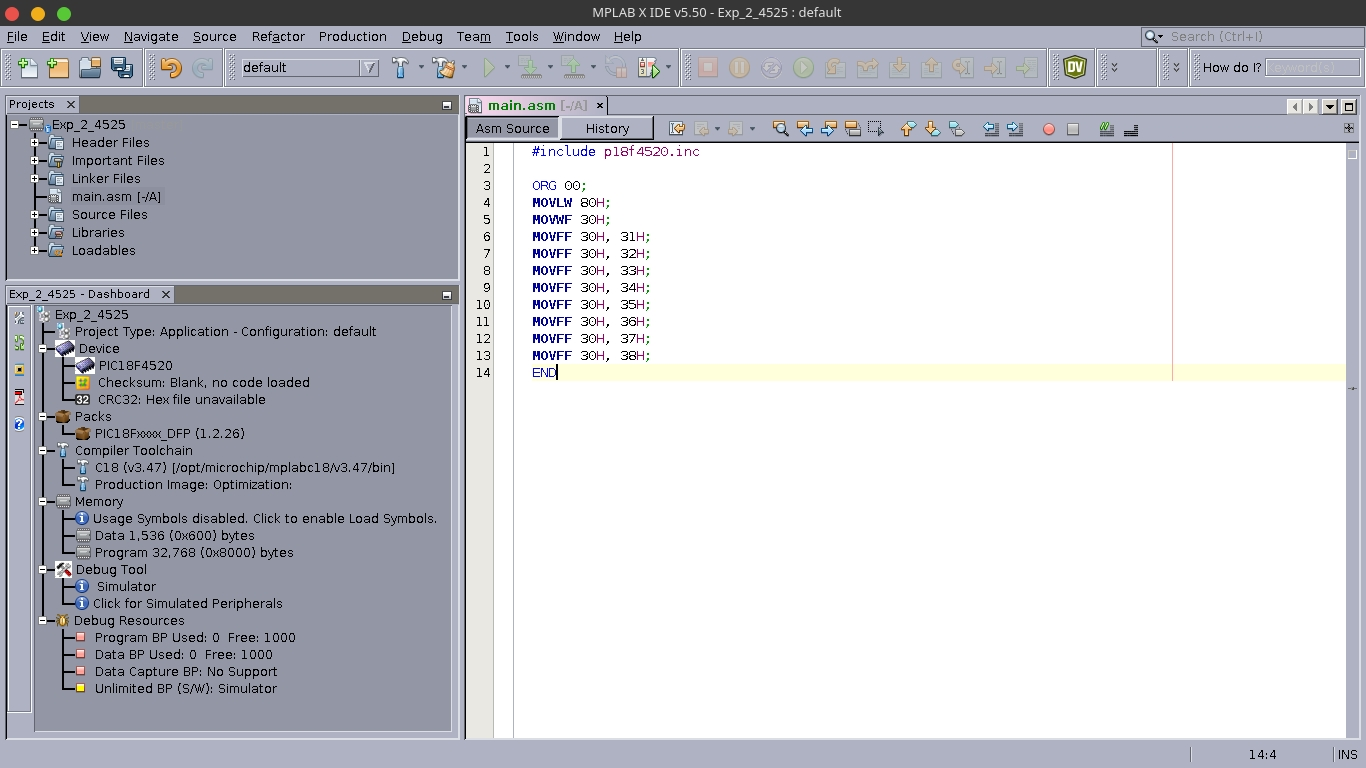
\includegraphics[width=0.85\textwidth]{private/1.png}
    \caption{Distribued Learning vs Federated Learning}
    \label{fig:dlVSfl}
\end{figure}

\par So, by this we can conclude that distributed learning focuses on scalable parallelized big data processing whereas, federated learning (FD) mainly focuses on processing distributed data on heterogeneous data sources.

\newpage
\subsection{The Steps in Federated Learning}
\begin{itemize}
    \item Identifying a problem to be solved
    \item Modifying the client’s application (optional)
    \item Simulating prototyping (optional)
    \item Training the federated model
    \item Evaluating the federated model
    \item Deploying FL at the server and clients. Thus, FL allows decreasing of:
    \begin{itemize}
        \item The risk of unauthorized data access, since data are not transmitted over the network
        \item Network traffic because the training results are usually much smaller in volume than the data themselves
        \item Time and cost of information transfer by reducing the amount of data transmitted
    \end{itemize}
    \item Requirements to the central computational cluster and the central storage, as there is no need to store all data in one place. At the same time, to implement FL, the following challenges must be solved: 
    \begin{itemize}
        \item Processing IID data as non-IID data, which can have different data partitions; 
        \item Working with clients with different computing and storage capacity, as well as scale and   stability; 
        \item Implementation of different communication schemes: centralized and decentralized; 
        \item Protection of transmitted analysis results from various types of attacks; 
        \item Aggregation of the results obtained from data sources to calculate inequality.
    \end{itemize}
\end{itemize}

\newpage
\subsection{Challanges of Federated Learning:}

\textbf{Data Partitioning:}

\par There are two different cases of how data are distributed in the IoT system.
\begin{itemize}
    \item Vertical partitioning: In this each storage node collects and stores data about different features of all objects.
    \item Horizontal partitioning: In this each storage node collects and stores data about all features of different objects.
\end{itemize}

\begin{figure}[!h]
    \centering
    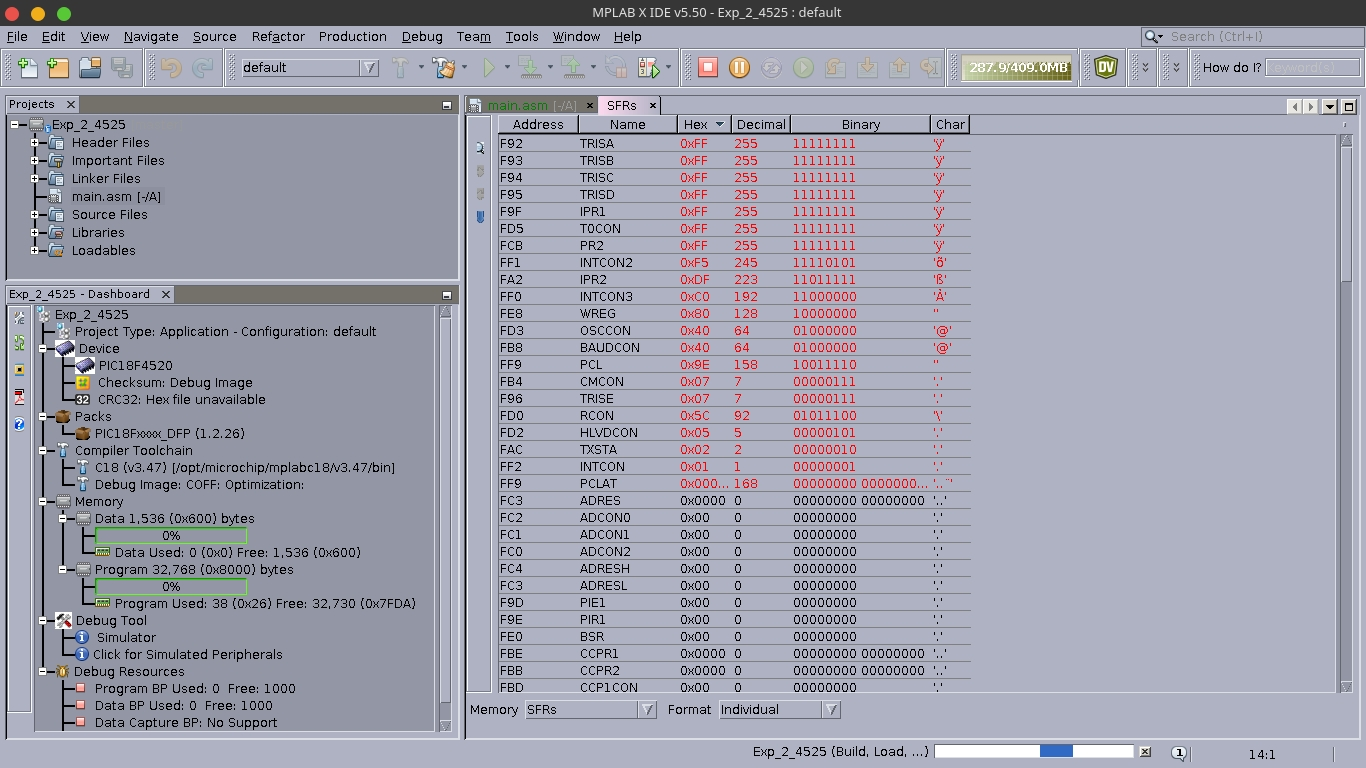
\includegraphics[width=0.75\textwidth]{private/2.png}
    \caption{Horizontal vs Vertical}
    \label{fig:hdpVSvdp}
\end{figure}

\textbf{Clients’ Settings:}
\par There are two different types of FL systems depending on the scale of federation.
\begin{itemize}
    \item Cross-silo systems have low scalable federation. They include organizations or data centers. Their numbers are small and rarely change.
    \item Cross-device systems have a scalable number of clients. They can be added and disabled at any moment of time. These are usually mobile devices and IoT devices.
\end{itemize}

\begin{figure}[!h]
    \centering
    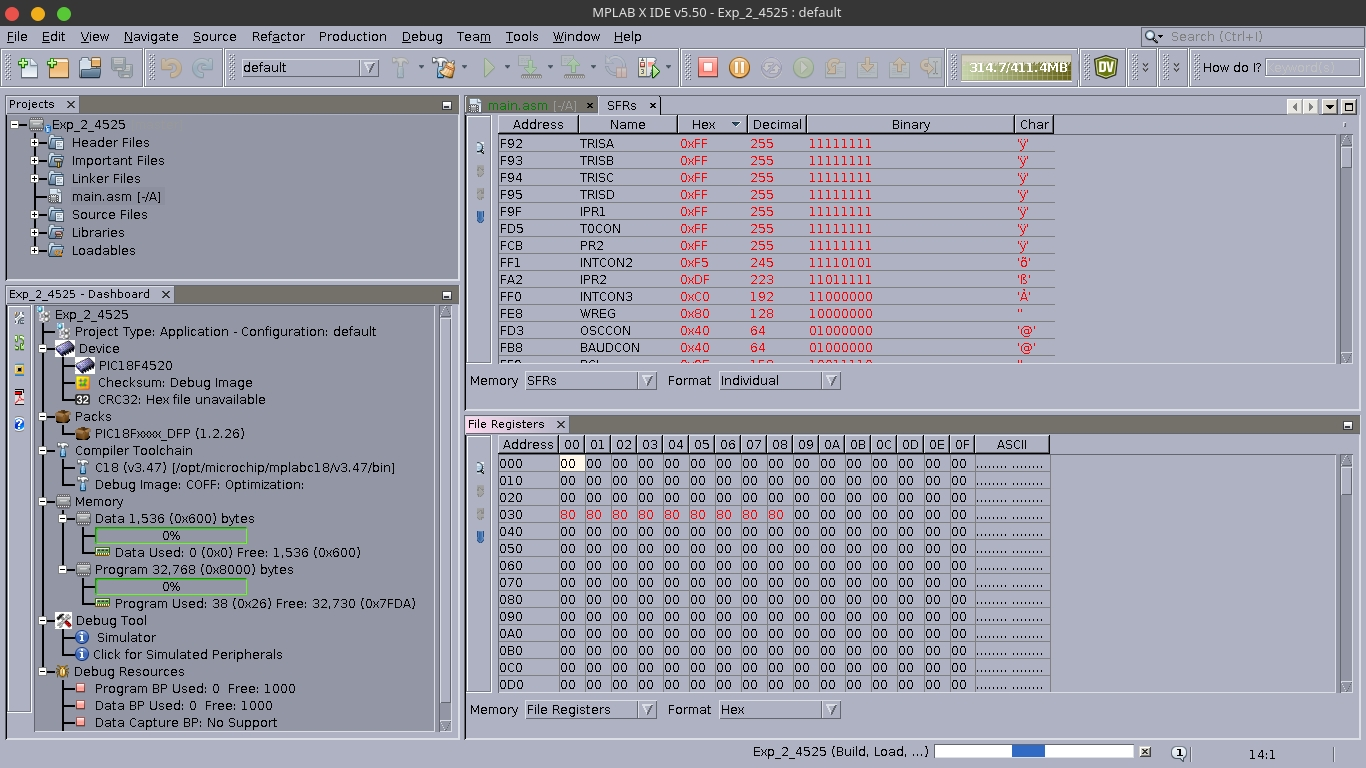
\includegraphics[width=0.75\textwidth]{private/3.png}
    \caption{Cross-Silo vs Cross-Device}
    \label{fig:cssiloVScsdev}
\end{figure}

\newpage
\textbf{Communication Schemes:}

\par FL systems can implement two communication schemes between their components centralized and decentralized.

\begin{itemize}
    \item The centralized scheme includes a central server. It is used to orchestrate different steps of the FL process and coordinate all clients therein. This scheme is typical for cross device systems. Since all selected nodes must send updates to a single entity, the server may become a bottleneck of the system.
    \item In the decentralized scheme, all clients can coordinate themselves to obtain the global model. This scheme is often used in cross-silo systems where clients have high-performance resources. Nevertheless, the specific network topology may affect the performance of the learning process.
\end{itemize}

\textbf{Data Privacy and Security Mechanisms:}

\par Data privacy and security are essential properties of FL. There is a need to secure the models and the analysis process to provide meaningful privacy guarantees. The attacks can be performed at all stages of the FL process and can target all FL elements.

\begin{itemize}
    \item Trained model
    \item Client
    \item Server
\end{itemize}

\par It is possible to outline two main types of FL-specific attacks—poisoning and inference attacks. The first type of attack aims to modify either the input data set or the parameters of the trained model in order to bias it in a way that is preferable to the adversary. The goal of inference attacks is to get access to personal or confidential data. Depending on the attack implementation mechanisms, it is possible to derive information about the properties of training data or the labels of training samples, or to determine if the sample was used in the training process. To protect FL against these attacks, the following security mechanisms are suggested: 
\par Secure multi-party computation (MPC) is a family of cryptographic protocols that allow a set of users to perform computations that use some private inputs without revealing them to other participants of the protocol. The most widely used implementations of MPC are the ABY3 and SecureML protocols. These protocols implement a server–aided computational model in which data owners send their data in encrypted format to a number of servers, usually two or three, which perform model training or apply a pre-trained model to analyze input data.

\textbf{Aggregation Algorithms}

\par One of the key issues of FL is aggregating model changes made by clients into a single model, as the aggregation function should not impair the accuracy of the model. The aggregation function depends on the model built in the FL process. For example, for centroid clusters constructed by the K-means algorithm, a prefix frequency filtering (PFF) method for data aggregation is suggested. 
\par To support energy and computationally efficient data aggregation of similar data sets, the authors applied the K-means clustering algorithm on the data and then aggregated the generated clusters using PFF. The ordered weighted averaging (OWA) algorithm was one of the first proposed for aggregating the weight coefficients of NNs. 
\par The aggregation of the parameters is based on the amount of data in every node. When calculating a regular average, each data point has an equal “weight”, i.e., it contributes equally to the final value. Weighted averages, on the other hand, weight each data point differently. Yager and Filev suggested a generalization of the OWA operator called the induced ordered weighted averaging (IOWA) operator. This operator firstly induces the ordering of arguments before their aggregation.
\newpage
\section{METHODOLOGY}
The following methodology will be followed to achieve the objectives defined for the proposed research work:
\begin{enumerate}
    \item Detailed study of Federated Learning frameworks for IoT will be done.
    \item Data will be generated in-house using various sensors and custom built devices for the training and simulation of FL.
    \item An in-depth study and Hands-on experience on existing approaches of Federated Learning will be done, to identify the Relative pros and cons for developing an efficient system
    \item Various Hardware and software-related parameters will be identified to evaluate the proposed system. 
    \item Data security and user privacy will be maintained.
    \item Comparison of our newly implemented approach with exsiting approaches will be done.
    \item Testing of the project by applying different conditions on it, so remove the remaining minorities in the project and to distinguish it in a better way. 
\end{enumerate}


\backmatter

\newpage
\addcontentsline{toc}{section}{TENTATIVE CHAPTER PLAN}
\section*{TENTATIVE CHAPTER PLAN}

\textbf{CHAPTER 1: INTRODUCTION }

\par This chapter introduces the reader to Federated learning and the basics of the project.

\textbf{CHAPTER 2: LITERATURE SURVEY}

\par This chapter includes the research already available for Applying Federated learning. The findings of the researchers will be highlighted which will become the basis of current implementation. And the existing and current approaches are compared. 

\textbf{CHAPTER 3: PROBLEM FORULATION}

\par This chapter covers the basic problem formulations and defines the solution as provided by the paper.

\textbf{CHAPTER 4: RESEARCH OBJECTIVES}

\par This chapter covers the main differences between distributed learning and federated learning. Also, it includes the steps and the challenges of federated learning, how we can use it and how we can overcome the challenges.
 
\textbf{CHAPTER 5: METHODOLOGY}

\par This chapter covers the technical details of the proposed approach. 

\textbf{REFERENCES}

\par This Section contains the references to other documents that are either useful or are directly reffered in this article.


\newpage
\addcontentsline{toc}{section}{REFERENCES}
\section*{REFERENCES}
\begin{enumerate}
    \item \par Santucci, G. From internet of data to internet of things. In Proceedings of the International Conference on Future Trends of the Internet, Luxembourg, 28 January 2009.
    \item \par Tsai, C.W.; Lai, C.F.; Vasilakos, A.V. Future Internet of Things: Open Issues and Challenges. Wirel. Netw. 2014, 20, 2201–2217.
    \item \par Atzori, L.; Iera, A.; Morabito, G. The internet of things: A survey. Comput. Netw. 2010, 54, 2787–2805.
    \item \par Gubbi, J.; Buyya, R.; Marusic, S.; Palaniswami, M. Internet of Things (IoT): A vision, architectural elements, and future directions. Future Gener. Comput. Syst. 2013, 29, 1645–1660. [CrossRef]
    \item \par Voigt, P.; Von dem Bussche, A. The EU general data protection regulation (GDPR). In A Practical Guide, 1st ed.; Springer International Publishing: Cham, Switzerland, 2017.
    \item \par California Consumer Privacy Act Home Page.
    \item \par Personal Data Protection Act 2012.
    \item \par Kairouz, P.; McMahan, H.B.; Avent, B.; Bellet, A.; Bennis, M.; Bhagoji, A.N.; d’Oliveira, R.G. Advances and open problems in federated learning. arXiv 2019, arXiv:1912.04977.
    \item \par Li, Q.; Wen, Z.; Wu, Z.; Hu, S.; Wang, N.; He, B. A Survey on Federated Learning Systems: Vision, Hype and Reality for Data Privacy and Protection. arXiv 2019, arXiv:1907.09693.
    \item \par Shokri, R.; Stronati, M.; Song, C.; Shmatikov, V. Membership Inference Attacks Against Machine Learning Models. In Proceedings of the IEEE Symposium on Security and Privacy (SP), San Jose, CA, USA, 22–24 May 2017; pp. 3–18. [CrossRef]
    \item \par Sun, G.; Cong, Y.; Dong, J.; Wang, Q.; Liu, J. Data Poisoning Attacks on Federated Machine Learning. arXiv 2020, arXiv:2004.10020.
    \item \par TensorFlow Federated: Machine Learning on Decentralized Data.
    \item \par Laulkar R,Daimiwal N2015 Application of Finger Photoplethysmography International Journal of Engineering Research and application volume 2., Issue 1,Jan-Feb 2015,pp.887-880
    \item \par Wei M,Chang R,Wang C, Lin C, Chen H 2016 Design of a Flexible PPG signal Process Wireless Device International Conference on Consumer Electronics-Taiwan
    \item \par Mohan P,Nagarjan V, Nisha A 2017 A frame work to estimate Heart Rate and Arterial Oxygen Saturation (Spo2) International Conference on Communication and Signal Processing April 6-8 2017 
    \item \par Xie Y,Gao Y,Lu W,Li W 2017 Development of Wearable Pulse Oximeter Based on Internet of Things and Signal Processing Techniques European Modelling Symposium 2017
\end{enumerate}

\end{document}